\chapter{El interior del átomo}\label{ch:g9:inside-the-atom}

En 1909, en un laboratorio de Mánchester, se lanzó un haz de partículas
diminutas y rápidas contra una lámina de pan de oro de unos pocos
cientos de \omterm{def:g7:atoms-and-molecules:atom}{átomos} de espesor. Casi todas la atravesaron en línea recta,
como si el oro estuviera vacío. Pero más o menos una de cada varios miles
rebotó. ``Era como si disparases un proyectil de quince pulgadas contra
un trozo de papel de seda y volviera y te diera'', dijo Ernest
Rutherford, cuyos alumnos habían hecho el experimento. El \omterm{def:g7:atoms-and-molecules:atom}{átomo}, el trozo
indivisible de materia, tenía una estructura, y estaba casi
completamente vacío.

\begin{recall}
Toda la materia está hecha de \omterm{def:g7:atoms-and-molecules:atom}{átomos}, de un centenar de clases
distintas, cada una con un símbolo como \ce{H}, \ce{C}, \ce{O}, \ce{Fe}.
Los \omterm{def:g7:atoms-and-molecules:atom}{átomos} se unen en \omterm{def:g7:atoms-and-molecules:molecule}{moléculas}, descritas por fórmulas como \ce{H2O}
(\cref{ch:g7:atoms-and-molecules}).
\end{recall}

\section{Núcleo y electrones}

\begin{definition}[Núcleo y electrón]\label{def:g9:inside-the-atom:nucleus}
Todo \omterm{def:g7:atoms-and-molecules:atom}{átomo} tiene un centro diminuto y pesado, el
\emph{núcleo}\index{nucleo@núcleo}, que lleva una carga eléctrica positiva. A
su alrededor se mueven unas partículas mucho más ligeras, los
\emph{electrones}\index{electron@electrón}, cada uno con la misma carga negativa,
$-e$.
\end{definition}

\begin{proposition}[Un átomo es neutro]\label{prop:g9:inside-the-atom:neutral}
% ledger: const:e
Un \omterm{def:g7:atoms-and-molecules:atom}{átomo} en su conjunto no tiene carga eléctrica: la carga positiva de
su \omterm{def:g9:inside-the-atom:nucleus}{núcleo} está exactamente compensada por las cargas negativas de sus
\omterm{def:g9:inside-the-atom:nucleus}{electrones}. La carga $e$ es diminuta: $e = \qty{1.60e-19}{C}$ (el
culombio, unidad de carga, pertenece al libro de física).
\end{proposition}

\begin{omfigure}
\begin{tikzpicture}[font=\small]
  \shade[inner color=omDef!35, outer color=white] (0,0) circle (2.2);
  \draw[omDef!60, dashed] (0,0) circle (2.2);
  \foreach \a/\r in {20/1.6,95/1.1,150/1.9,215/1.4,290/1.7,340/0.9} {
    \fill[omDef] (\a:\r) circle (0.06);
    \node[font=\scriptsize, omDef] at ($(\a:\r)+(0.18,0.16)$) {$-$};
  }
  \fill[red!70!black] (0,0) circle (0.1);
  \draw[<-, omProp, thick] (-0.12,0.02) -- (-3.0,0.9) node[left, text=black, align=right]
    {núcleo: diminuto,\\ pesado, positivo};
  \draw[<-, omProp, thick] ($(20:1.6)+(0.08,0.02)$) -- (3.0,0.9) node[right, text=black]
    {un electrón: ligero, negativo};
  \draw[<-, omProp, thick] (300:2.2) -- (3.0,-1.4) node[right, text=black, align=left]
    {los electrones se mueven en una nube\\ alrededor del núcleo};
\end{tikzpicture}

{\small Un \omterm{def:g7:atoms-and-molecules:atom}{átomo}, sin respetar la escala. Si el \omterm{def:g9:inside-the-atom:nucleus}{núcleo} se dibujara del
tamaño del punto rojo, la nube de \omterm{def:g9:inside-the-atom:nucleus}{electrones} mediría unos cientos de
metros.}
\end{omfigure}

\section{Protones y neutrones}

\begin{definition}[Protón, neutrón, nucleón]\label{def:g9:inside-the-atom:proton}
El \omterm{def:g9:inside-the-atom:nucleus}{núcleo} está formado por dos clases de partículas: los
\emph{protones}\index{proton@protón}, cada uno con la carga $+e$, y los
\emph{neutrones}\index{neutron@neutrón}, que no tienen carga. Los protones y
los neutrones, que tienen casi la misma masa, se llaman en conjunto
\emph{nucleones}\index{nucleon@nucleón}.
\end{definition}

\begin{definition}[Número atómico y número másico]\label{def:g9:inside-the-atom:atomic-number}
El número de \omterm{def:g9:inside-the-atom:proton}{protones} de un \omterm{def:g9:inside-the-atom:nucleus}{núcleo} es el \emph{número
atómico}\index{numero atomico@número atómico}, que se escribe $Z$. El número de
\omterm{def:g9:inside-the-atom:proton}{nucleones} (\omterm{def:g9:inside-the-atom:proton}{protones} y \omterm{def:g9:inside-the-atom:proton}{neutrones} juntos) es el
\emph{número másico}\index{numero masico@número másico}, que se escribe $A$. El
número de \omterm{def:g9:inside-the-atom:proton}{neutrones} es $N = A - Z$.
\end{definition}

\begin{notation}[El símbolo del núclido]\label{not:g9:inside-the-atom:symbol}
Un \omterm{def:g7:atoms-and-molecules:atom}{átomo} con un \omterm{def:g9:inside-the-atom:nucleus}{núcleo} dado se escribe con su símbolo, el \omterm{def:g9:inside-the-atom:atomic-number}{número másico}
arriba a la izquierda y el \omterm{def:g9:inside-the-atom:atomic-number}{número atómico} abajo a la izquierda:
\ce{^{A}_{Z}X}. Por ejemplo, \ce{^{12}_{6}C} tiene 6 \omterm{def:g9:inside-the-atom:proton}{protones} y $12 - 6 =
6$ \omterm{def:g9:inside-the-atom:proton}{neutrones}; \ce{^{56}_{26}Fe} tiene 26 \omterm{def:g9:inside-the-atom:proton}{protones} y 30 \omterm{def:g9:inside-the-atom:proton}{neutrones}.
\end{notation}

\begin{method}[Leer el símbolo de un núclido]\label{met:g9:inside-the-atom:read}
Para \ce{^{A}_{Z}X}:
\begin{enumerate}
  \item \omterm{def:g9:inside-the-atom:proton}{protones}: $Z$;
  \item \omterm{def:g9:inside-the-atom:proton}{neutrones}: $A - Z$;
  \item \omterm{def:g9:inside-the-atom:nucleus}{electrones} del \omterm{def:g7:atoms-and-molecules:atom}{átomo} neutro: $Z$, los mismos que \omterm{def:g9:inside-the-atom:proton}{protones}.
\end{enumerate}
Para \ce{^{23}_{11}Na}: 11 \omterm{def:g9:inside-the-atom:proton}{protones}, 12 \omterm{def:g9:inside-the-atom:proton}{neutrones}, 11 \omterm{def:g9:inside-the-atom:nucleus}{electrones}.
\end{method}

\begin{omfigure}
\begin{tikzpicture}[font=\small]
  \node[font=\Huge, inner sep=1pt] (x) at (0,0) {\ce{^{35}_{17}Cl}};
  \draw[<-, omProp, thick, shorten <=3pt] ([xshift=5pt,yshift=-7pt]x.north west) -- (-2.6,1.0)
    node[left, text=black, align=right] {número másico $A = 35$:\\ protones + neutrones};
  \draw[<-, omProp, thick, shorten <=3pt] ([xshift=5pt,yshift=7pt]x.south west) -- (-2.6,-1.0)
    node[left, text=black, align=right] {número atómico $Z = 17$:\\ protones};
  \draw[<-, omProp, thick] ([xshift=2pt]x.east) -- (2.2,0) node[right, text=black,
    align=left] {símbolo del elemento:\\ cloro};
\end{tikzpicture}

{\small Lectura del símbolo de un núclido: este \omterm{def:g7:atoms-and-molecules:atom}{átomo} de cloro tiene 17
\omterm{def:g9:inside-the-atom:proton}{protones}, $35 - 17 = 18$ \omterm{def:g9:inside-the-atom:proton}{neutrones} y, si es neutro, 17 \omterm{def:g9:inside-the-atom:nucleus}{electrones}.}
\end{omfigure}

\section{El elemento químico y sus isótopos}

\begin{definition}[Elemento químico]\label{def:g9:inside-the-atom:element}
Un \emph{elemento químico}\index{elemento quimico@elemento químico} es el conjunto de
todos los \omterm{def:g7:atoms-and-molecules:atom}{átomos}, y de todos los \omterm{def:g7:atoms-and-molecules:atom}{átomos} con carga que se forman a partir
de ellos, que tienen el mismo \omterm{def:g9:inside-the-atom:atomic-number}{número atómico} $Z$. Cada elemento tiene
un nombre y un símbolo: todo \omterm{def:g7:atoms-and-molecules:atom}{átomo} con 6 \omterm{def:g9:inside-the-atom:proton}{protones} es un \omterm{def:g7:atoms-and-molecules:atom}{átomo} de
carbono, \ce{C}; todo \omterm{def:g7:atoms-and-molecules:atom}{átomo} con 8 \omterm{def:g9:inside-the-atom:proton}{protones} es un \omterm{def:g7:atoms-and-molecules:atom}{átomo} de oxígeno,
\ce{O}.
\end{definition}

\begin{definition}[Isótopos]\label{def:g9:inside-the-atom:isotope}
Los \omterm{def:g7:atoms-and-molecules:atom}{átomos} de un mismo elemento que tienen distinto número de
\omterm{def:g9:inside-the-atom:proton}{neutrones}, y por tanto distinto \omterm{def:g9:inside-the-atom:atomic-number}{número másico}, son
\emph{isótopos}\index{isotopo@isótopo} de ese elemento. Tienen el mismo $Z$ y
distinto $A$.
\end{definition}

\begin{example}[Isótopos del carbono y del hidrógeno]\label{ex:g9:inside-the-atom:isotopes}
% ledger: iso:C12, iso:C13, iso:H2
El carbono natural tiene alrededor de un \qty{98.9}{\percent} de
carbono~12, \ce{^{12}_{6}C}, y un \qty{1.1}{\percent} de carbono~13,
\ce{^{13}_{6}C}, con una traza de carbono~14, \ce{^{14}_{6}C}, cuya
lenta transformación en otro \omterm{def:g9:inside-the-atom:nucleus}{núcleo} sirve para datar maderas y huesos
antiguos (la radiactividad pertenece al libro de física). El hidrógeno
tiene tres \omterm{def:g9:inside-the-atom:isotope}{isótopos}: \ce{^{1}_{1}H}, sin ningún \omterm{def:g9:inside-the-atom:proton}{neutrón}, con mucho el
más abundante; el deuterio \ce{^{2}_{1}H}, unos pocos \omterm{def:g7:atoms-and-molecules:atom}{átomos} de cada
cien mil; y el tritio \ce{^{3}_{1}H}.
\end{example}

\begin{proposition}[Los isótopos se comportan igual en química]\label{prop:g9:inside-the-atom:alike}
La química de un \omterm{def:g7:atoms-and-molecules:atom}{átomo} depende de sus \omterm{def:g9:inside-the-atom:nucleus}{electrones}, y los \omterm{def:g9:inside-the-atom:isotope}{isótopos} de un
elemento tienen el mismo número de \omterm{def:g9:inside-the-atom:nucleus}{electrones}. Por tanto, los \omterm{def:g9:inside-the-atom:isotope}{isótopos}
reaccionan de la misma manera: el agua hecha con deuterio tiene casi
exactamente el mismo aspecto y el mismo comportamiento que el agua
ordinaria.
\end{proposition}

\begin{omfigure}
\begin{tikzpicture}[font=\small, p/.style={circle, inner sep=0pt, minimum size=4.2mm,
    ball color=red!65}, n/.style={circle, inner sep=0pt, minimum size=4.2mm,
    ball color=black!20}]
  \node[p] at (0,0) {};
  \node[anchor=north, align=center] at (0,-0.45) {\ce{^{1}_{1}H}\\ 1 protón};
  \node[p] at (3.0,0) {}; \node[n] at (3.35,0.1) {};
  \node[anchor=north, align=center] at (3.2,-0.45) {\ce{^{2}_{1}H}\\ 1 protón, 1 neutrón};
  \node[p] at (6.4,0) {}; \node[n] at (6.75,0.12) {}; \node[n] at (6.55,0.35) {};
  \node[anchor=north, align=center] at (6.6,-0.45) {\ce{^{3}_{1}H}\\ 1 protón, 2 neutrones};
  \node[draw=black!30, fill=red!65, circle, minimum size=3mm, inner sep=0pt] at (9.1,0.2) {};
  \node[anchor=west] at (9.3,0.2) {protón};
  \node[draw=black!30, fill=black!20, circle, minimum size=3mm, inner sep=0pt] at (9.1,-0.3) {};
  \node[anchor=west] at (9.3,-0.3) {neutrón};
\end{tikzpicture}

{\small Los \omterm{def:g9:inside-the-atom:nucleus}{núcleos} de los tres \omterm{def:g9:inside-the-atom:isotope}{isótopos} del hidrógeno: un \omterm{def:g9:inside-the-atom:proton}{protón} cada
uno, y 0, 1 o 2 \omterm{def:g9:inside-the-atom:proton}{neutrones}.}
\end{omfigure}

\section{Tamaños y masas}

\begin{proposition}[El núcleo es diminuto y contiene casi toda la masa]\label{prop:g9:inside-the-atom:sizes}
% ledger: const:a0, r:proton, const:mp, const:mn, const:me
Un \omterm{def:g7:atoms-and-molecules:atom}{átomo} mide alrededor de \qty{e-10}{m} de diámetro; su \omterm{def:g9:inside-the-atom:nucleus}{núcleo}, entre
\qty{e-15}{m} y \qty{e-14}{m}: entre diez mil y cien mil veces menos.
Las masas de las partículas son
\[
  m_p = \qty{1.673e-27}{kg},\qquad m_n = \qty{1.675e-27}{kg},\qquad
  m_e = \qty{9.11e-31}{kg}.
\]
Un \omterm{def:g9:inside-the-atom:proton}{protón} es unas 1836 veces más pesado que un \omterm{def:g9:inside-the-atom:nucleus}{electrón}, así que más del
\qty{99.9}{\percent} de la masa de un \omterm{def:g7:atoms-and-molecules:atom}{átomo} está en su \omterm{def:g9:inside-the-atom:nucleus}{núcleo}.
\end{proposition}

\begin{example}[Una canica en un estadio]\label{ex:g9:inside-the-atom:marble}
Si el \omterm{def:g9:inside-the-atom:nucleus}{núcleo} de un \omterm{def:g7:atoms-and-molecules:atom}{átomo} fuera una canica de \qty{1}{cm} de diámetro, el
\omterm{def:g7:atoms-and-molecules:atom}{átomo} mediría alrededor de $\qty{1}{cm} \times 100\,000 = \qty{1}{km}$:
una canica en el centro de un estadio enorme, con unas motas de polvo
(los \omterm{def:g9:inside-the-atom:nucleus}{electrones}) girando alrededor de las gradas. La materia es, sobre
todo, espacio vacío.
\end{example}

\begin{method}[La masa de un átomo]\label{met:g9:inside-the-atom:mass}
Como los \omterm{def:g9:inside-the-atom:proton}{protones} y los \omterm{def:g9:inside-the-atom:proton}{neutrones} tienen casi la misma masa y los
\omterm{def:g9:inside-the-atom:nucleus}{electrones} son muy ligeros, la masa de un \omterm{def:g7:atoms-and-molecules:atom}{átomo} se acerca a $A \times
\qty{1.67e-27}{kg}$, donde $A$ es su \omterm{def:g9:inside-the-atom:atomic-number}{número másico}. Un \omterm{def:g7:atoms-and-molecules:atom}{átomo} de
carbono~12:
$12 \times 1.67 \times 10^{-27} = \qty{2.00e-26}{kg}$.
\end{method}

\section{Breve historia del modelo atómico}

\begin{history}[De lo indivisible al núcleo, 1897--1932]
En 1897, J.~J.~Thomson descubrió el \omterm{def:g9:inside-the-atom:nucleus}{electrón}, una partícula mucho más
ligera que cualquier \omterm{def:g7:atoms-and-molecules:atom}{átomo}: después de todo, los \omterm{def:g7:atoms-and-molecules:atom}{átomos} sí se podían
dividir. Imaginó el \omterm{def:g7:atoms-and-molecules:atom}{átomo} como una bola de materia positiva salpicada de
\omterm{def:g9:inside-the-atom:nucleus}{electrones}. En 1909--1911, el experimento de la lámina de oro del equipo
de Rutherford mostró que la carga positiva y casi toda la masa se
encuentran en un \omterm{def:g9:inside-the-atom:nucleus}{núcleo} diminuto. En 1913, Niels Bohr propuso que los
\omterm{def:g9:inside-the-atom:nucleus}{electrones} ocupan niveles de energía fijos a su alrededor, y en 1932
James Chadwick descubrió el \omterm{def:g9:inside-the-atom:proton}{neutrón}.
\end{history}

\begin{omfigure}
\begin{minipage}[b]{0.3\linewidth}\centering
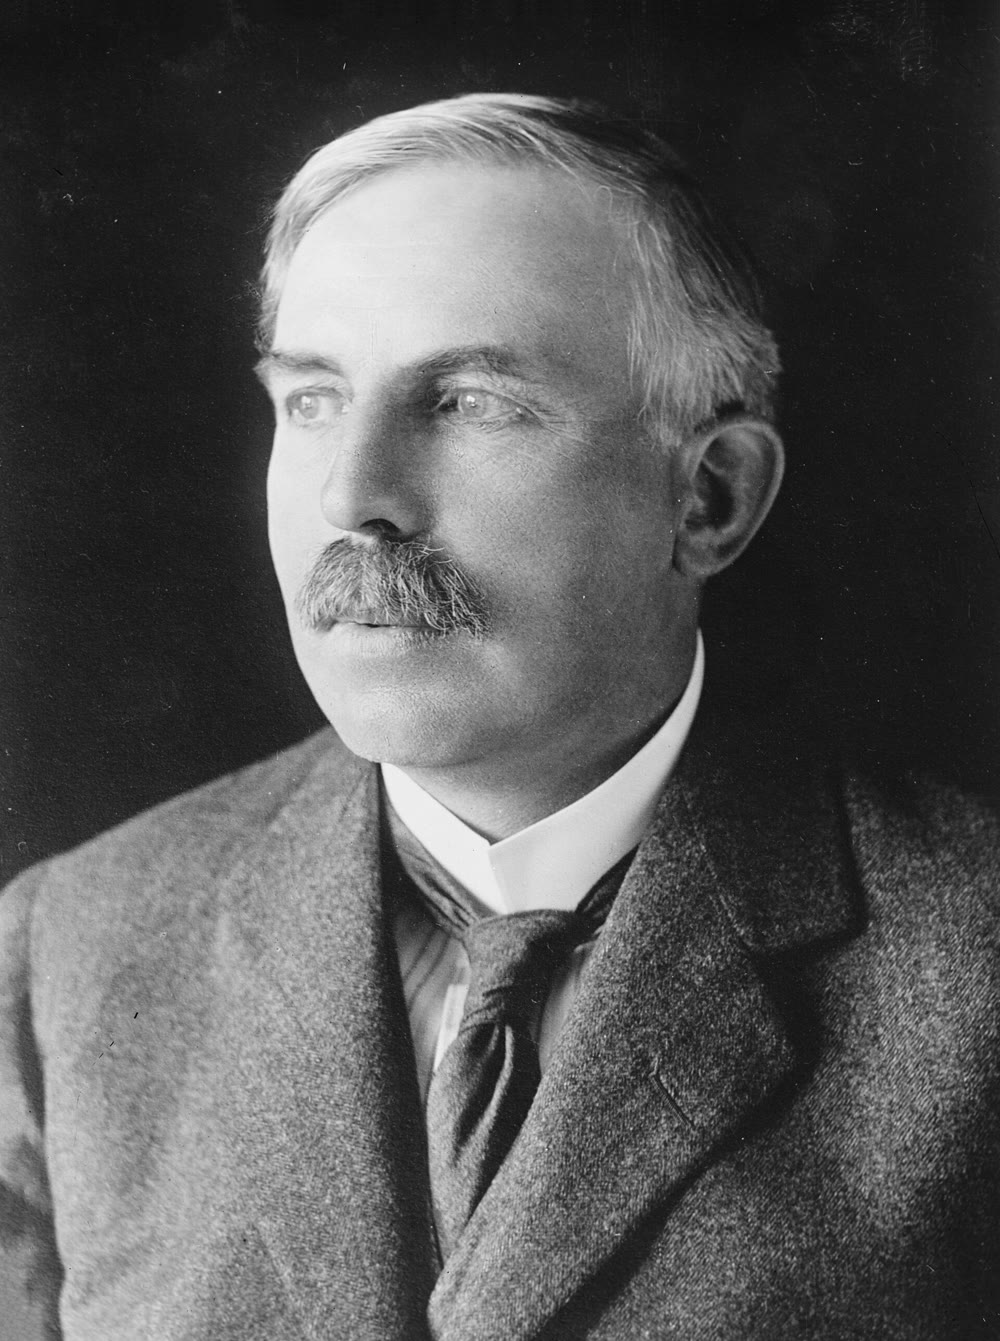
\includegraphics[width=\linewidth]{images/book1/rutherford.jpg}

{\small Ernest Rutherford (1871--1937).}
\end{minipage}\hfill
\begin{minipage}[b]{0.66\linewidth}\centering
\begin{tikzpicture}[font=\small]
  \fill[black!45] (0,-0.5) rectangle (0.9,0.5);
  \node[anchor=north, align=center] at (0.45,-0.55) {fuente de\\ partículas alfa};
  \draw[->, thick, red!70!black] (0.9,0) -- (2.8,0);
  \fill[yellow!70!orange] (2.8,-1.6) rectangle (2.88,1.6);
  \node[anchor=north] at (2.84,-1.65) {lámina de oro};
  \draw[omDef!40, line width=4pt] (5.6,-1.8) arc[start angle=-30, end angle=30, radius=3.6];
  \foreach \y in {-0.3,-0.1,0.1,0.3} \draw[->, red!70!black] (2.88,\y) -- (5.3,\y);
  \draw[->, red!70!black] (2.88,0.05) -- (5.0,1.15);
  \draw[->, red!70!black] (2.88,-0.05) -- (4.9,-1.3);
  \draw[->, red!70!black, thick] (2.8,0.02) .. controls (2.2,0.35) .. (1.6,0.95);
  \node[anchor=west, align=left, font=\footnotesize] at (6.25,0) {la mayoría\\ pasan\\ de largo};
  \node[anchor=south, align=center, font=\footnotesize] at (1.6,1.0) {muy pocas\\ rebotan};
\end{tikzpicture}

{\small El experimento de la lámina de oro: la mayoría de las partículas
la atraviesan en línea recta; unas pocas se desvían; muy pocas rebotan
contra un \omterm{def:g9:inside-the-atom:nucleus}{núcleo}.}
\end{minipage}
\end{omfigure}

\section{Ejercicios}

\begin{exercise}[$\star$]\label{exo:g9:inside-the-atom:1}
Nombra las partículas del \omterm{def:g9:inside-the-atom:nucleus}{núcleo} y las partículas que lo rodean, con el
signo de su carga.
\end{exercise}

\begin{exercise}[$\star$]\label{exo:g9:inside-the-atom:2}
Da el número de \omterm{def:g9:inside-the-atom:proton}{protones}, \omterm{def:g9:inside-the-atom:proton}{neutrones} y \omterm{def:g9:inside-the-atom:nucleus}{electrones} de \ce{^{16}_{8}O},
\ce{^{27}_{13}Al} y \ce{^{40}_{20}Ca}.
\end{exercise}

\begin{exercise}[$\star$]\label{exo:g9:inside-the-atom:3}
¿Por qué un \omterm{def:g7:atoms-and-molecules:atom}{átomo} es eléctricamente neutro?
\end{exercise}

\begin{exercise}[$\star$]\label{exo:g9:inside-the-atom:4}
Un \omterm{def:g7:atoms-and-molecules:atom}{átomo} tiene 26 \omterm{def:g9:inside-the-atom:proton}{protones} y 30 \omterm{def:g9:inside-the-atom:proton}{neutrones}. Escribe el símbolo de su
núclido (el elemento es el hierro, \ce{Fe}).
\end{exercise}

\begin{exercise}[$\star\star$]\label{exo:g9:inside-the-atom:5}
¿Son \ce{^{35}_{17}Cl} y \ce{^{37}_{17}Cl} el mismo elemento? ¿Son
\omterm{def:g9:inside-the-atom:isotope}{isótopos}? Explícalo.
\end{exercise}

\begin{exercise}[$\star\star$]\label{exo:g9:inside-the-atom:6}
¿Son \omterm{def:g9:inside-the-atom:isotope}{isótopos} \ce{^{14}_{6}C} y \ce{^{14}_{7}N}? Explícalo.
\end{exercise}

\begin{exercise}[$\star\star$]\label{exo:g9:inside-the-atom:7}
Calcula, en notación científica, la masa aproximada de un \omterm{def:g7:atoms-and-molecules:atom}{átomo} de
\ce{^{56}_{26}Fe}.
\end{exercise}

\begin{exercise}[$\star\star$]\label{exo:g9:inside-the-atom:8}
En el experimento de la lámina de oro, ¿por qué la mayoría de las
partículas atraviesan el oro en línea recta?
\end{exercise}

\begin{exercise}[$\star\star$]\label{exo:g9:inside-the-atom:9}
¿Cuántas veces más pequeño que un \omterm{def:g7:atoms-and-molecules:atom}{átomo} (\qty{e-10}{m}) es un \omterm{def:g9:inside-the-atom:nucleus}{núcleo} de
\qty{e-15}{m}? Escribe la respuesta como una potencia de diez.
\end{exercise}

\begin{exercise}[$\star\star$]\label{exo:g9:inside-the-atom:10}
¿Por qué los \omterm{def:g9:inside-the-atom:isotope}{isótopos} de un elemento tienen la misma química?
\end{exercise}

\begin{exercise}[$\star\star\star$]\label{exo:g9:inside-the-atom:11}
Un \omterm{def:g7:atoms-and-molecules:atom}{átomo} de hierro tiene 26 \omterm{def:g9:inside-the-atom:nucleus}{electrones}. Calcula su masa total y, después,
la fracción de la masa de un \omterm{def:g7:atoms-and-molecules:atom}{átomo} de \ce{^{56}_{26}Fe} que representan
(usa la masa hallada en el ejercicio~7).
\end{exercise}

\begin{exercise}[$\star\star\star$]\label{exo:g9:inside-the-atom:12}
% ledger: iso:Cu63, iso:Cu65
El cobre natural tiene un \qty{69.15}{\percent} de cobre~63 y un
\qty{30.85}{\percent} de cobre~65. De cada 10\,000 \omterm{def:g7:atoms-and-molecules:atom}{átomos} de cobre,
¿cuántos son de cada \omterm{def:g9:inside-the-atom:isotope}{isótopo}? ¿Cuál es el número medio de \omterm{def:g9:inside-the-atom:proton}{nucleones} por
\omterm{def:g7:atoms-and-molecules:atom}{átomo} de cobre?
\end{exercise}

\clearpage % mantiene el título junto al recuadro del problema (quedaba aislado al pie de una página)
\section{Problema: Pesar el cloro}

\begin{problem}[{Problema de fin de semana --- dos isótopos del cloro,
la masa de cada átomo y la masa media de un átomo de cloro}]
\label{pb:g9:inside-the-atom:1}
% ledger: iso:Cl35, iso:Cl37, const:me, const:mp, const:mn
El cloro natural es una \omterm{def:g6:pure-substances-and-mixtures:mixture}{mezcla} de dos \omterm{def:g9:inside-the-atom:isotope}{isótopos}, el cloro~35 y el
cloro~37: de cada 1000 \omterm{def:g7:atoms-and-molecules:atom}{átomos} de cloro, unos 758 son de cloro~35 y 242
de cloro~37. Toma como masa de un \omterm{def:g9:inside-the-atom:proton}{nucleón} \qty{1.67e-27}{kg} y como
masa de un \omterm{def:g9:inside-the-atom:nucleus}{electrón} \qty{9.11e-31}{kg}. El \omterm{def:g9:inside-the-atom:atomic-number}{número atómico} del cloro es
17.

\medskip
\noindent\textbf{Parte I --- Dos \omterm{def:g9:inside-the-atom:nucleus}{núcleos}.}
\begin{enumerate}
  \item Escribe los símbolos de los núclidos de los dos \omterm{def:g9:inside-the-atom:isotope}{isótopos}.
  \item Da el número de \omterm{def:g9:inside-the-atom:proton}{protones}, \omterm{def:g9:inside-the-atom:proton}{neutrones} y \omterm{def:g9:inside-the-atom:nucleus}{electrones} de cada uno.
  \item ¿Por qué los dos se llaman cloro? ¿Por qué son \omterm{def:g9:inside-the-atom:isotope}{isótopos}?
  \item ¿Reaccionará con el sodio una muestra de cloro~37 igual que una
        muestra de cloro~35? Explícalo.
\end{enumerate}

\medskip
\noindent\textbf{Parte II --- La masa de cada \omterm{def:g7:atoms-and-molecules:atom}{átomo}.}
\begin{enumerate}[resume]
  \item Calcula la masa del \omterm{def:g9:inside-the-atom:nucleus}{núcleo} de un \omterm{def:g7:atoms-and-molecules:atom}{átomo} de cloro~35.
  \item Calcula la masa de los 17 \omterm{def:g9:inside-the-atom:nucleus}{electrones}, y comprueba que se puede
        despreciar al lado del \omterm{def:g9:inside-the-atom:nucleus}{núcleo}.
  \item Calcula la masa de un \omterm{def:g7:atoms-and-molecules:atom}{átomo} de cloro~37.
  \item ¿Cuántos \omterm{def:g7:atoms-and-molecules:atom}{átomos} de cloro~35 pesarían \qty{1}{g}? Da la respuesta
        en notación científica.
\end{enumerate}

\medskip
\noindent\textbf{Parte III --- El \omterm{def:g7:atoms-and-molecules:atom}{átomo} medio.}
\begin{enumerate}[resume]
  \item ¿Qué porcentaje de los \omterm{def:g7:atoms-and-molecules:atom}{átomos} de cloro son de cloro~35? ¿Y de
        cloro~37?
  \item En 1000 \omterm{def:g7:atoms-and-molecules:atom}{átomos} de cloro natural, calcula la masa total de los
        \omterm{def:g7:atoms-and-molecules:atom}{átomos} de cloro~35 y la de los \omterm{def:g7:atoms-and-molecules:atom}{átomos} de cloro~37.
  \item Calcula la masa de esos 1000 \omterm{def:g7:atoms-and-molecules:atom}{átomos}.
  \item Deduce la masa media de un \omterm{def:g7:atoms-and-molecules:atom}{átomo} de cloro.
\end{enumerate}
\end{problem}
